% ============================================================
%  Lab 3: Proximal Policy Optimization (PPO) on Enduro-v5
%  編譯方式：XeLaTeX（Overleaf：Menu -> Compiler -> XeLaTeX）
%  圖片放在 figures/ 資料夾
% ============================================================
\documentclass[11pt,a4paper]{article}

\usepackage[margin=2.2cm]{geometry}
\usepackage{fontspec}
\usepackage{xeCJK}
% [字型] Overleaf 有 Noto Serif CJK TC；Windows 本機編譯則退回微軟正黑體
\IfFontExistsTF{Noto Serif CJK TC}{
  \setCJKmainfont{Noto Serif CJK TC}
  \setCJKsansfont{Noto Sans CJK TC}
  \setCJKmonofont{Noto Sans CJK TC}
}{
  \setCJKmainfont{Microsoft JhengHei}
  \setCJKsansfont{Microsoft JhengHei}
  \setCJKmonofont{Microsoft JhengHei}
}
\xeCJKsetup{CJKspace=true}

\usepackage{amsmath,amssymb}
\usepackage{graphicx}
\usepackage{booktabs}
\usepackage{array}
\usepackage{multirow}
\usepackage{float}
\usepackage{caption}
\usepackage{subcaption}
\usepackage{enumitem}
\usepackage{xcolor}
\usepackage{listings}
\usepackage[hidelinks]{hyperref}

\captionsetup{font=small,labelfont=bf}
\setlist{itemsep=2pt,topsep=4pt}
\renewcommand{\arraystretch}{1.15}
\linespread{1.15}

\lstset{
  basicstyle=\ttfamily\footnotesize,
  keywordstyle=\color{blue!60!black},
  commentstyle=\color{gray},
  frame=single, rulecolor=\color{gray!50},
  breaklines=true, columns=fullflexible, language=Python,
  xleftmargin=4pt, xrightmargin=4pt
}

% [圖片] 有 TensorBoard 截圖就用截圖 (#1)，否則用 matplotlib 匯出的同一份資料 (#2)
\newcommand{\figOr}[3]{%
  \IfFileExists{figures/#1}{\includegraphics[width=#3]{figures/#1}}{\includegraphics[width=#3]{figures/#2}}}

% ===== 請填入 =====
\newcommand{\studentid}{314513067}
\newcommand{\studentname}{張晉堯}
% ==================

\title{\textbf{Lab 3: Proximal Policy Optimization (PPO)}\\[2pt]\large Selected Topics in Reinforcement Learning, Fall 2026}
\author{\studentid\quad \studentname}
\date{}

\begin{document}
\maketitle
\vspace{-1.5em}

\begin{center}
\fbox{\begin{minipage}{0.92\linewidth}
\textbf{結果摘要}
\begin{itemize}[leftmargin=1.2em]
  \item 依助教 sample code 實作 PPO-clip + GAE，先以助教超參數訓練 20M steps（baseline）：seed 0--19 的 greedy 平均 788，最遠到第 4 天。
  \item 之後以「分段降低學習率」續訓（$2.5\times10^{-4}\rightarrow10^{-5}\rightarrow10^{-6}$，其餘超參數不變），並用短探測決定降學習率的時機，共 77.8M steps。
  \item 最終模型 seed 0--19 平均 \textbf{1920}，5 場測試平均 \textbf{1910.4}；固定 seed 12 可重現 \textbf{2339 分、第 9 天}（評分表最高級）。
\end{itemize}
\end{minipage}}
\end{center}

% ============================================================
\section{實作說明}
% ============================================================

\subsection{環境前處理}
\begin{itemize}[leftmargin=1.2em]
  \item \texttt{gym.make("ALE/Enduro-v5", frameskip=1)} 後接 \texttt{AtariPreprocessing}：
        no-op reset（最多 30 步）、frame skip 4（取最後兩幀的 max）、灰階、resize 成 $84\times84$。
        v5 預設本身有 frame skip 4，所以在 \texttt{gym.make} 設 \texttt{frameskip=1}，避免跳兩次。sticky action 0.25 維持 v5 預設。
  \item \texttt{FrameStack(4)}：觀測為 $(4, 84, 84)$ 的 uint8，網路中除以 255。
  \item Reward clipping：存進 buffer 給 PPO 學習的 reward 取 $\mathrm{sign}(r)\in\{-1,0,1\}$；
        TensorBoard 的 \texttt{Train/Episode Reward}、評估與測試都使用原始 reward。
\end{itemize}

\subsection{網路架構（sample code）}
Actor 與 critic 共用 CNN（Nature DQN 架構），各接一個 head：
\[
(4,84,84)\xrightarrow{\text{Conv }8\times8,\,32,\,s4}\xrightarrow{\text{Conv }4\times4,\,64,\,s2}\xrightarrow{\text{Conv }3\times3,\,64,\,s1}3136
\;\Rightarrow\;
\begin{cases}
\text{Actor: FC 512}\rightarrow 9 \text{ logits}\\
\text{Critic: FC 512}\rightarrow V(s)
\end{cases}
\]
權重採 orthogonal initialization（sample code 為 gain $\sqrt2$），另將 actor 輸出層設為 gain 0.01（初始 policy 接近均勻分布）、critic 輸出層 gain 1。

\subsection{選擇動作與 forward}
Forward 以 logits 建立 $\pi_\theta(\cdot|s)=\mathrm{Categorical}(\text{logits})$，回傳 action、$\log\pi_\theta(a|s)$、$V(s)$、entropy：
\begin{itemize}[leftmargin=1.2em]
  \item 收集資料時從分布取樣（探索）；評估與測試時取 $\arg\max$（greedy）；
  \item update 時傳入 buffer 中的動作 $a$，計算新 policy 下該動作的 log probability。
\end{itemize}
\texttt{decide\_agent\_actions} 將觀測加上 batch 維度 $(1,4,84,84)$，在 \texttt{torch.no\_grad()} 下 forward，並把 $a_t$、$V(s_t)$、$\log\pi_{\theta_\text{old}}(a_t|s_t)$ 存入 buffer。

\subsection{GAE}
助教的 \texttt{GaeSampleMemory} 把每條 trajectory 切成 horizon $=128$ 的片段，由後往前計算
\[
\delta_t = r_t + \gamma V(s_{t+1})(1-d_t) - V(s_t),\qquad
\hat A_t = \delta_t + \gamma\lambda(1-d_t)\hat A_{t+1},\qquad
\hat R_t = \hat A_t + V(s_t),
\]
片段尾端以 $V(s_{t+128})$ bootstrap，episode 結束（$d_t=1$）時不 bootstrap。$\hat R_t$ 作為 critic 的目標。

\subsection{PPO 更新}
每收集 10000 步更新一次：資料打亂後切成 128 筆的 minibatch，共 3 個 epoch（每次 update 約 $3\times79=237$ 次梯度步），更新完清空 buffer。每個 minibatch：
\begin{align*}
r_t(\theta) &= \exp\big(\log\pi_\theta(a_t|s_t)-\log\pi_{\theta_\text{old}}(a_t|s_t)\big),\qquad
\tilde A_t = \frac{\hat A_t-\mu_{\hat A}}{\sigma_{\hat A}+10^{-8}}\ \text{（minibatch 內正規化）}\\
L^{\text{CLIP}} &= -\,\mathbb{E}_t\Big[\min\big(r_t\tilde A_t,\ \mathrm{clip}(r_t,1-\epsilon,1+\epsilon)\tilde A_t\big)\Big],\qquad
L^{V} = \mathbb{E}_t\big[(V_\theta(s_t)-\hat R_t)^2\big]\\
L &= L^{\text{CLIP}} + c_v L^{V} - c_e\,\mathbb{E}_t\big[\mathcal{H}[\pi_\theta(\cdot|s_t)]\big]
\end{align*}
反向傳播後做 gradient norm clipping（0.5）再以 Adam 更新。另外在 TensorBoard 記錄 approx KL $\mathbb{E}[(r_t-1)-\log r_t]$ 與 clip fraction（$|r_t-1|>\epsilon$ 的比例），用來觀察每次更新的幅度。

\begin{lstlisting}
_, logp_new, value_new, entropy = self.net(ob_train_batch, a=ac_train_batch)
adv_train_batch = (adv_train_batch - adv_train_batch.mean()) / (adv_train_batch.std() + 1e-8)
ratio = torch.exp(logp_new - logp_pi_train_batch)
surr1 = ratio * adv_train_batch
surr2 = torch.clamp(ratio, 1.0 - self.clip_epsilon, 1.0 + self.clip_epsilon) * adv_train_batch
surrogate_loss = -torch.min(surr1, surr2).mean()
v_loss = value_criterion(value_new, return_train_batch)   # nn.MSELoss()
entropy = entropy.mean()
loss = surrogate_loss + self.value_coefficient * v_loss - self.entropy_coefficient * entropy
self.optim.zero_grad()
loss.backward()
nn.utils.clip_grad_norm_(self.net.parameters(), self.max_gradient_norm)
self.optim.step()
\end{lstlisting}

\subsection{超參數}
\begin{table}[H]
\centering\small
\begin{tabular}{ll@{\hspace{3em}}ll}
\toprule
Batch size & 128 & Optimizer & Adam \\
Learning rate & $2.5\times10^{-4}$（\S\ref{sec:lr} 分段降低） & Gamma $\gamma$ & 0.99 \\
Lambda $\lambda$ & 0.95 & Value coefficient $c_v$ & 0.5 \\
Entropy coefficient $c_e$ & 0.01 & Update epoch & 3 \\
Clip $\epsilon$ & 0.2 & Max gradient norm & 0.5 \\
Horizon & 128 & Update every & 10000 steps \\
Evaluation & 每 500k steps，3 場 greedy & 環境數 & 1 \\
\bottomrule
\end{tabular}
\caption{超參數。除了 \S\ref{sec:lr} 的學習率之外，全部使用助教給定的數值。}
\end{table}

% ============================================================
\section{實驗結果}
% ============================================================

\subsection{Baseline：助教超參數，20M steps}
單一環境訓練 20,000,472 steps，約 16.8 小時（含評估，平均 330 steps/s）。評估分數在前 2.5M 步都是 0，3M 步開始上升（5M：241、8M：430），13M 之後在 460--780 之間震盪。

\begin{figure}[H]
\centering
\begin{subfigure}{0.49\linewidth}\centering
  \figOr{tb_baseline_train.png}{baseline_train_reward.png}{\linewidth}
  \caption{Train/Episode Reward}
\end{subfigure}\hfill
\begin{subfigure}{0.49\linewidth}\centering
  \figOr{tb_baseline_eval.png}{baseline_eval_reward.png}{\linewidth}
  \caption{Evaluate/Episode Reward（3 場平均）}
\end{subfigure}
\caption{Baseline（lr $2.5\times10^{-4}$，0--20M steps）的訓練曲線，reward 皆為原始分數。}
\label{fig:baseline}
\end{figure}

訓練中評估只有 3 場，雜訊很大：評估最高的 15.0M checkpoint（776.3）在 seed 0--19 上平均只有 553.9；
最後的 20M checkpoint 平均 788.1，20 個 seed 中 7 個到第 4 天，是 baseline 中實際最強的模型。

\subsection{分段降低學習率續訓}
\label{sec:lr}
\paragraph{動機。}
Baseline 末期每次 update 的 approx KL 約 0.04、clip fraction 約 0.3，代表在 lr $2.5\times10^{-4}$ 下 policy 每次更新都移動不少，
評估分數也一直震盪。參考往年修課同學的做法（$2.5\times10^{-4}$ 訓練 100M $\rightarrow$ $10^{-5}$ 40M $\rightarrow$ $10^{-6}$ 60M），
其曲線顯示降學習率後的前 2M 步就大幅跳升，之後收益很小。由於時間只夠約 1/3 的步數，我改用「短探測」決定何時降學習率：

\begin{enumerate}[leftmargin=1.5em]
  \item \textbf{主線}：從 baseline 20M 的 checkpoint（含 Adam 狀態）以 lr $2.5\times10^{-4}$ 繼續訓練。
  \item \textbf{探測}：在 20M / 35M / 50M / 65M 從主線分支，改用 lr $10^{-5}$ 訓練 3M steps（與主線並行）。
  \item \textbf{評分}：分支點與探測結束都以 seed 0--19 各測 1 場（greedy），取平均。不使用訓練中只有 3 場的評估。
  \item \textbf{停損}：若探測分數比前一個探測進步不到 100（約 1/3 天），就停止主線。
  \item \textbf{收尾}：分數最高的探測以 $10^{-5}$ 延長到「分支點 + 10M」，再以 $10^{-6}$ 訓練 3M steps。
\end{enumerate}

\begin{table}[H]
\centering\small
\begin{tabular}{cccccc}
\toprule
分支點 & 主線（$2.5\times10^{-4}$） & 降到 $10^{-5}$ 訓練 3M 後 & 降學習率的增幅 & 比前一個探測 & 決策 \\
\midrule
20M & 788.1 & 1114.8 & +326.6 & -- & 繼續 \\
35M & 1008.2 & 1214.9 & +206.7 & +100.1 & 繼續 \\
50M & 796.4 & 1551.8 & +755.4 & +336.9 & 繼續 \\
65M & 1367.5 & 1585.1 & +217.6 & +33.2 & \textbf{停止主線} \\
\bottomrule
\end{tabular}
\caption{各分支點的 seed 0--19 greedy 平均分數。}
\label{tab:probe}
\end{table}

\begin{figure}[H]
\centering
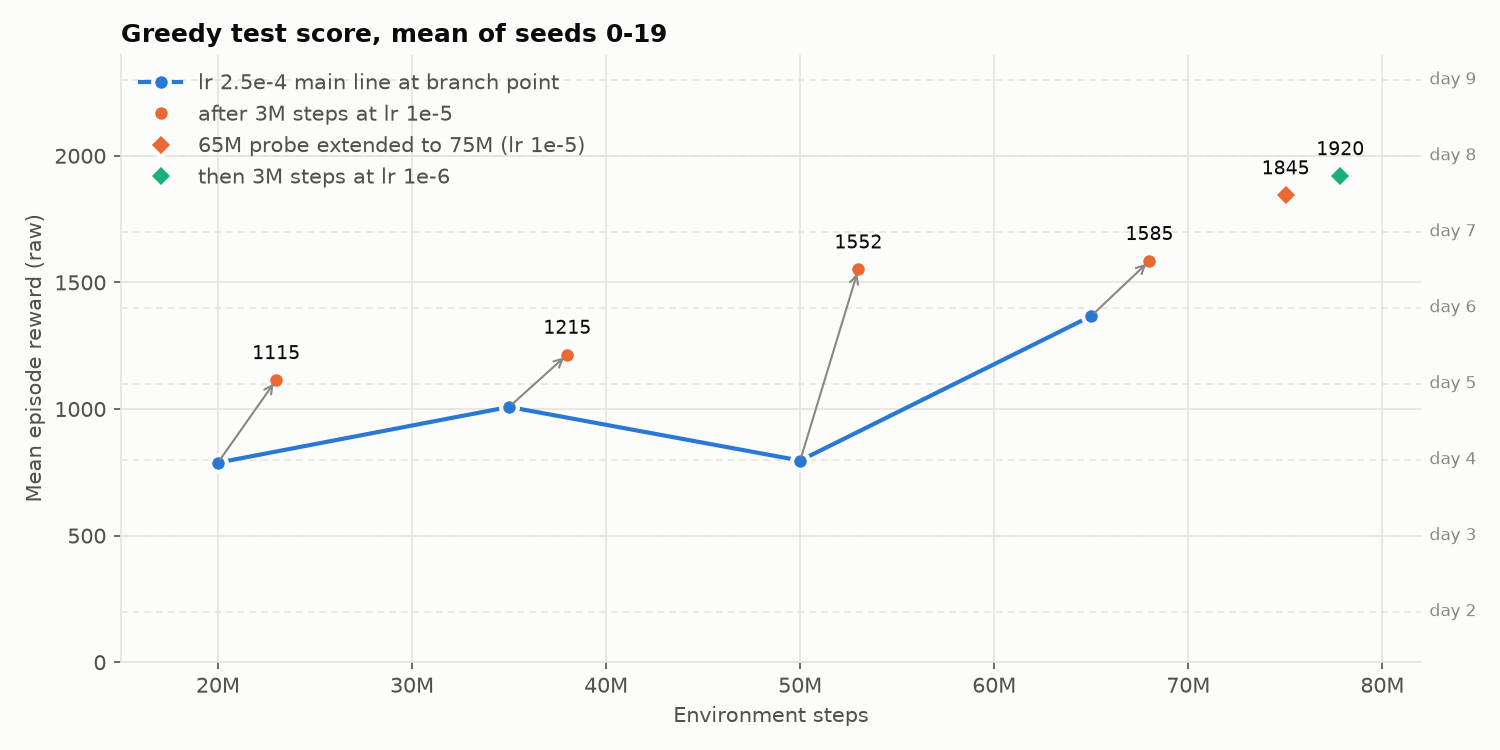
\includegraphics[width=0.75\linewidth]{figures/lr_decay_probe_scores.png}
\caption{藍點：主線在分支點的分數；橘點：降到 $10^{-5}$ 訓練 3M steps 後的分數；菱形：收尾階段。虛線為評分表的天數分界。}
\label{fig:probe}
\end{figure}

\begin{table}[H]
\centering\small
\begin{tabular}{lcccc}
\toprule
模型 & 總步數 & seed 0--19 平均 & 天數分布（場數） & 第 9 天 \\
\midrule
Baseline（$2.5\times10^{-4}$） & 20.0M & 788.1 & 第 2--4 天 & 0 \\
65M 探測（$10^{-5}$，3M） & 68.0M & 1585.1 & 第 4--8 天 & 0 \\
延長（$10^{-5}$） & 75.0M & 1844.6 & 4:2, 5:1, 6:3, 7:10, 8:4 & 0 \\
\textbf{再接 $10^{-6}$ 3M（最終）} & \textbf{77.8M} & \textbf{1920.3} & 5:4, 6:1, 7:9, 8:2, 9:4 & \textbf{4} \\
\bottomrule
\end{tabular}
\caption{收尾階段結果。最終模型的學習率排程為 0--65M：$2.5\times10^{-4}$，65--74.8M：$10^{-5}$，74.8--77.8M：$10^{-6}$。}
\label{tab:final}
\end{table}

\begin{figure}[H]
\centering
\begin{subfigure}{0.495\linewidth}\centering
  \figOr{tb_lr_decay_train.png}{lr_decay_train_reward.png}{\linewidth}
  \caption{Train/Episode Reward}
\end{subfigure}\hfill
\begin{subfigure}{0.495\linewidth}\centering
  \figOr{tb_lr_decay_eval.png}{lr_decay_eval_reward.png}{\linewidth}
  \caption{Evaluate/Episode Reward（3 場平均）}
\end{subfigure}
\caption{所有學習率階段的 TensorBoard 訓練曲線（每個實驗一條曲線，接在分支點之後）：
0--20M 為 baseline，20--68.4M 為 lr $2.5\times10^{-4}$ 續訓的主線；
20/35/50/65M 開始的短曲線為 lr $10^{-5}$ 的探測（65M 的探測延長到 75M）；最後 74.8--77.8M 為 lr $10^{-6}$。}
\label{fig:lr_curves}
\end{figure}

\paragraph{觀察。}
\begin{itemize}[leftmargin=1.2em]
  \item 每次降學習率都立刻大幅加分（+207 至 +755），而且 3M steps 內就看得出來，和參考曲線一致。
  \item 主線本身的分數震盪很大（50M 的 796 比 35M 的 1008 還低），但從它分出的探測分數持續上升，所以「降學習率後再測」比直接看主線可靠。
  \item 降到 $10^{-5}$ 後 approx KL 從約 0.04 降到約 0.004，clip fraction 從約 0.27 降到約 0.04；$10^{-6}$ 時 KL 約 $3\times10^{-5}$，policy 幾乎不再改變。
        這段只多了 76 分，在 seed 雜訊範圍內，但到第 9 天的 seed 從 0 個變成 4 個。
  \item 主線在 68.4M 停止。總共 77.8M steps 就達到第 9 天，主要省在用 3M steps 的探測取代長時間的低學習率訓練。
\end{itemize}

\subsection{測試結果（5 games）}
最終模型（\texttt{Enduro\_lr1e-5\_from65M\_then\_lr1e-6/model\_77830590\_1533.pth}），greedy，起始 seed 12：

\begin{figure}[H]
\centering
\figOr{test_5games_screenshot.png}{test_5games_seed12.png}{0.72\linewidth}
\caption{5 場測試結果（\texttt{python test.py --episodes 5 --seed 12}）。只有第 1 場以 seed 12 reset，第 2--5 場接續同一個 RNG。}
\label{fig:test}
\end{figure}

\begin{table}[H]
\centering\small
\begin{tabular}{lcccccc}
\toprule
模型 & Ep 1 & Ep 2 & Ep 3 & Ep 4 & Ep 5 & 平均 \\
\midrule
Baseline 20M（seed 0） & 948 & 928 & 949 & 764 & 780 & 873.8 \\
最終 77.8M（seed 0） & 1387 & 1380 & 1919 & 1846 & 1846 & 1675.6 \\
最終 77.8M（seed 12） & 2339 & 1687 & 1986 & 1656 & 1884 & \textbf{1910.4} \\
\bottomrule
\end{tabular}
\caption{5 場測試的原始 reward。}
\end{table}

\subsection{Demo 設定}
最終模型在 seed 0--19 中有 4 個 seed 到第 9 天，各自單獨執行 \texttt{test.py --episodes 1 --seed N} 的結果與掃描完全相同：

\begin{figure}[H]
\centering
\begin{minipage}[c]{0.55\linewidth}\centering\small
\begin{tabular}{ccccc}
\toprule
Seed & Length & Total reward & 天數 & 評分表分數 \\
\midrule
\textbf{12} & \textbf{26997} & \textbf{2339} & \textbf{9} & \textbf{50} \\
19 & 26993 & 2327 & 9 & 50 \\
10 & 26994 & 2323 & 9 & 50 \\
6 & 26995 & 2322 & 9 & 50 \\
\bottomrule
\end{tabular}
\captionof{table}{第 9 天的 seed（greedy）。長度約 27000 是撞到 108000 frames 的上限被截斷，在時間限制內已經玩到第 9 天。}
\end{minipage}\hfill
\begin{minipage}[c]{0.36\linewidth}\centering

\includegraphics[width=0.75\linewidth]{figures/demo_seed12_last_frame.png}
\caption{seed 12 錄影的最後一格：儀表板顯示第 9 天（剩 261 台）。}
\end{minipage}
\end{figure}

Demo 指令（\texttt{--render} 為即時顯示；\texttt{--record} 存影片）：
\begin{lstlisting}
python test.py --exp-name Enduro_lr1e-5_from65M_then_lr1e-6 --ckpt ../runs/Enduro_lr1e-5_from65M_then_lr1e-6/checkpoints/model_77830590_1533.pth --episodes 1 --seed 12 --render
\end{lstlisting}

% ============================================================
\section{問題回答}
% ============================================================

\subsection*{Q1. PPO is an on-policy or an off-policy algorithm? Why?}
PPO 是 \textbf{on-policy} 演算法。
\begin{itemize}[leftmargin=1.2em]
  \item PPO 的目標函數是對「目前 policy $\pi_{\theta_\text{old}}$ 收集的資料」取期望：
        \[L^{\text{CLIP}}(\theta)=\mathbb{E}_{(s_t,a_t)\sim\pi_{\theta_\text{old}}}\big[\min(r_t\hat A_t,\ \mathrm{clip}(r_t,1-\epsilon,1+\epsilon)\hat A_t)\big].\]
        Advantage $\hat A_t$ 也是用目前的 critic 在這批軌跡上算出來的，只對產生資料的那個 policy 有意義。
  \item 每一輪先用 $\pi_{\theta_\text{old}}$ 收集資料，用這批資料更新幾個 epoch 後就丟掉，再用新的 policy 重新收集。
        實作中 buffer 每收集 10000 步就做 3 個 epoch 的 update，然後 \texttt{clear\_buffer()}，不會重複使用舊 policy 的資料。
  \item Ratio $r_t=\pi_\theta/\pi_{\theta_\text{old}}$ 是 importance sampling，但只用來修正同一輪 update 中 $\theta$ 偏離 $\theta_\text{old}$ 的小差距。
        若拿很久以前的 policy 的資料來用，ratio 會非常大或非常小，變異數爆炸，也大多會被 clip 掉而沒有梯度，所以不能像 off-policy 方法那樣重複使用舊資料。
  \item 相對地，DQN 是 off-policy：它的 target $r+\gamma\max_{a'}Q(s',a')$ 與產生資料的行為策略無關，所以可以用 replay buffer 反覆抽取很久以前的經驗。
\end{itemize}
嚴格來說，同一批資料做多個 epoch 時，第 2、3 個 epoch 的 $\pi_\theta$ 已經和收集資料的 $\pi_{\theta_\text{old}}$ 有些不同，這是靠 ratio 與 clipping 處理的「輕微 off-policy」；但整體而言，PPO 仍是只使用最新 policy 資料的 on-policy 方法。

\subsection*{Q2. How does PPO ensure that policy updates at each step are not too large?}
\begin{enumerate}[leftmargin=1.5em]
  \item \textbf{Clipped surrogate objective（核心）}：
  \[
  L^{\text{CLIP}}=\mathbb{E}_t\big[\min\big(r_t\hat A_t,\ \mathrm{clip}(r_t,1-\epsilon,1+\epsilon)\hat A_t\big)\big],\quad \epsilon=0.2 .
  \]
  \begin{itemize}[leftmargin=1.2em]
    \item $\hat A_t>0$（好動作）：$r_t$ 超過 $1+\epsilon$ 後目標不再增加，沒有誘因把該動作的機率提高超過 20\%。
    \item $\hat A_t<0$（壞動作）：$r_t$ 低於 $1-\epsilon$ 後目標不再增加，不會把機率壓得太低。
    \item 取 $\min$ 讓目標成為未截斷目標的悲觀下界：改壞的方向不會被截斷（仍會被懲罰），改好的方向則有上限。
          被截斷的樣本梯度為 0，所以 policy 一旦離 $\pi_{\theta_\text{old}}$ 太遠，這些樣本就不再推動它。
  \end{itemize}
  這是 TRPO 的 KL 信任區域（$\mathbb{E}[\mathrm{KL}(\pi_{\theta_\text{old}}\|\pi_\theta)]\le\delta$）的一階近似，不需要二階最佳化。
  \item \textbf{有限的更新量}：每批資料只做 3 個 epoch、minibatch 128，加上較小的 learning rate，限制了每輪 policy 能移動的距離。
  \item \textbf{Gradient norm clipping（0.5）}：限制單一梯度步的大小，避免少數極端樣本造成大跳動。
  \item \textbf{Advantage 正規化}：minibatch 內把 $\hat A$ 標準化，讓不同時期的更新尺度一致。
  \item \textbf{Entropy bonus 與 value loss}：entropy 項防止 policy 太快變成 deterministic；critic 穩定則 advantage 估計穩定，間接讓更新穩定。
\end{enumerate}
需要注意的是，clipping 並不是硬性保證：在本實驗中，lr $2.5\times10^{-4}$ 時每次 update 的 approx KL 約 0.04、clip fraction 約 0.3，policy 仍移動不少，評估分數也明顯震盪；
學習率降到 $10^{-5}$ 後，KL 降到約 0.004、clip fraction 約 0.04，分數立刻大幅提升（表~\ref{tab:probe}）。
所以實務上常再配合 learning rate annealing 或 KL early stopping，進一步控制更新幅度。

\subsection*{Q3. Why is GAE-$\lambda$ used instead of one-step advantages? How does it help policy learning?}
\begin{itemize}[leftmargin=1.2em]
  \item \textbf{One-step advantage} $\hat A_t^{(1)}=\delta_t=r_t+\gamma V(s_{t+1})-V(s_t)$：變異數低，但完全依賴 critic 的估計，\textbf{偏差（bias）大}。
        訓練初期 critic 幾乎是隨機的，one-step advantage 的訊號主要是 critic 的誤差；而且獎勵只能透過 $V$ 一步一步往前傳，credit assignment 很慢。
  \item \textbf{Monte Carlo advantage} $\sum_l\gamma^l r_{t+l}-V(s_t)$：對 critic 誤差無偏，但累加整條軌跡的隨機性，\textbf{變異數大}。
        Enduro 的 episode 長達 3000--27000 步，加上 sticky action 的隨機性，梯度會非常吵。
  \item \textbf{GAE} 是所有 $k$-step advantage 的指數加權平均：
  \[
  \hat A_t^{\text{GAE}(\gamma,\lambda)}=\sum_{l=0}^{\infty}(\gamma\lambda)^l\,\delta_{t+l}
  =(1-\lambda)\big(\hat A_t^{(1)}+\lambda\hat A_t^{(2)}+\lambda^2\hat A_t^{(3)}+\cdots\big).
  \]
  它用 $\lambda$ 在兩者之間連續地取捨 bias 與 variance。
\end{itemize}
對 policy learning 的幫助：
\begin{enumerate}[leftmargin=1.5em]
  \item 變異數較低的 policy gradient 讓每次更新的方向更可靠，同樣的樣本能學得更穩、更有效率（PPO 每批資料只用 3 個 epoch，樣本效率很重要）。
  \item 偏差比 one-step 小，獎勵能在一次計算中往前傳好幾十步，做出較正確的 credit assignment。
        例如 Enduro 中「轉向閃車」的決策在幾幀之後才得到超車的 +1，GAE 能把這個訊號直接歸給之前的動作。
  \item $\hat R_t=\hat A_t+V(s_t)$ 就是 TD($\lambda$) return，也提供 critic 一個 bias 與 variance 較平衡的訓練目標，critic 學得好又回過頭讓 advantage 更準。
  \item 可以用固定長度的片段（horizon 128）截斷計算，片段尾端用 $V$ bootstrap，不必等 episode 結束，適合 Enduro 這種很長的 episode。
\end{enumerate}

\subsection*{Q4. What does $\lambda$ represent in GAE-$\lambda$, and how does adjusting it affect PPO?}
$\lambda\in[0,1]$ 是 GAE 對未來 TD error 的衰減係數，代表「要相信實際觀察到的多步回報到什麼程度，又要多依賴 critic 的估計」：
\begin{align*}
\lambda=0&:\ \hat A_t=\delta_t &&\text{（one-step TD：低變異、高偏差）}\\
\lambda=1&:\ \hat A_t=\textstyle\sum_l\gamma^l r_{t+l}-V(s_t) &&\text{（Monte Carlo：無偏、高變異）}
\end{align*}
$(\gamma\lambda)^l$ 決定第 $l$ 步之後的 TD error 還有多少權重，等效的估計長度約為 $1/(1-\gamma\lambda)$。
本實驗 $\gamma=0.99,\lambda=0.95$，$1/(1-0.9405)\approx16.8$ 個 agent step（約 67 幀，約 1.1 秒的遊戲時間），
而 horizon 128 處的權重 $(0.9405)^{128}\approx4\times10^{-4}$，所以片段截斷對估計幾乎沒有影響。

調整 $\lambda$ 的影響：
\begin{itemize}[leftmargin=1.2em]
  \item \textbf{$\lambda$ 調小（如 0.8 以下）}：更依賴 critic，advantage 變異數小、前期更新平穩，
        但 critic 不準時偏差大，policy 可能朝錯誤方向優化或收斂到較差的解；長期的獎勵傳播也變慢。
  \item \textbf{$\lambda$ 調大（接近 1）}：更依賴實際回報，偏差小、能捕捉較長期的後果，
        但變異數大，需要更多樣本或更小的學習率，訓練曲線也較不穩。對 Enduro 這種很長、隨機性高（sticky action）的 episode 影響更明顯。
  \item \textbf{實務上}：常用 0.9--0.97，0.95 是 PPO 論文與 Atari 常用的折衷值。$\lambda$ 和 $\gamma$ 一起決定有效的回報長度，critic 越準就越能用較小的 $\lambda$。
\end{itemize}
本實驗沒有調整 $\lambda$（固定 0.95），以上是依理論與 GAE 的 bias--variance 分析推論的影響。

% ============================================================
\section{其他觀察}
% ============================================================
\begin{itemize}[leftmargin=1.2em]
  \item \textbf{3 場評估不可靠}：20M checkpoint 在 seed 0--19 的單場分數從 473 到 994 都有。用訓練中 3 場評估選出的 \texttt{best.pth}（15.0M）實際上比最後的 20M checkpoint 差約 230 分。
        因此本實驗的決策都用 20 個固定 seed 的平均。
  \item \textbf{Greedy 優於隨機取樣}：Baseline 末期 entropy 約 1.2（9 個動作的最大值為 $\ln 9\approx2.2$），隨機取樣常做出錯誤動作；
        20M checkpoint 的 greedy 平均 788，取樣平均只有 600，所以評估與測試都用 $\arg\max$。
  \item \textbf{可重現性}：測試時固定 torch / numpy / 環境的 seed，並關閉 cuDNN 的非確定性演算法，同一個 seed 的結果完全相同（包含開啟錄影時）。
  \item \textbf{卡關模式}：Baseline 的 episode 長度幾乎都是一天的整數倍（6650 / 9980 / 13310），代表 agent 都是在某天結束時差一點沒達標；
        降低學習率後，同樣的 policy 架構可以穩定撐到第 7--9 天。
\end{itemize}

% ============================================================
\begin{thebibliography}{9}
\bibitem{ppo} J. Schulman, F. Wolski, P. Dhariwal, A. Radford, O. Klimov. Proximal Policy Optimization Algorithms. arXiv:1707.06347, 2017.
\bibitem{gae} J. Schulman, P. Moritz, S. Levine, M. Jordan, P. Abbeel. High-Dimensional Continuous Control Using Generalized Advantage Estimation. ICLR, 2016.
\bibitem{trpo} J. Schulman, S. Levine, P. Moritz, M. Jordan, P. Abbeel. Trust Region Policy Optimization. ICML, 2015.
\bibitem{dqn} V. Mnih et al. Playing Atari with Deep Reinforcement Learning. arXiv:1312.5602, 2013.
\bibitem{37} S. Huang et al. The 37 Implementation Details of Proximal Policy Optimization. ICLR Blog Track, 2022.
\bibitem{gym} OpenAI. Gym Documentation: Enduro. \url{https://www.gymlibrary.dev/environments/atari/enduro/}
\end{thebibliography}

\end{document}
